\section{Evaluation}
In this section, we show the feasibility of the approach of using declarative
analysis for multilingual program, and the effectiveness of its
implentation. More specifically, we set three research questions as follow:

RQ1) Feasibility: Is it possible to implement a working static analyzer for multilingual program in declarative style?

RQ2) Performance: How is the spped and precision of implemented analyzer, compared to the state-of-the-art analyzer?

RQ3) Usefulness: How practical is the implemented analyzer?

To answer RQ1, we ran our implemented analyzer to NativeFlowBench, which is a
small set of becnhmarks manually crafted by authors of JN-SAF[2], with the
purpose of testing dataflow analyzer for JNI programs. It consists of 23
android applications featuring various interactions between C++ and Java, some
of which contain a malicious code pattern that tries leak sensitive user data.
To answer RQ2, we ran our analyzer to 42 real-world android applications
collected from F-Droid[9], a repository for open-source android application. These
42 apps are selected by searching for apps with JNI, and among them, selecting those
that we could sucessfully compile. We compared our analyzer with
state-of-the-art[3] JNI analyzer, and confirmed that our analyzer outperforms
in terms of scalability and precision.  To answer RQ3, we implemented various
kinds of bug checkers, illustrated in previous researches[1][3], on top of our
analyzer. We ran our bug checker on the 42 applications of F-Droid mentioned
above, and discovered 38 bugs, including 30 newly found bugs.


\subsection{RQ1: Feasibility}
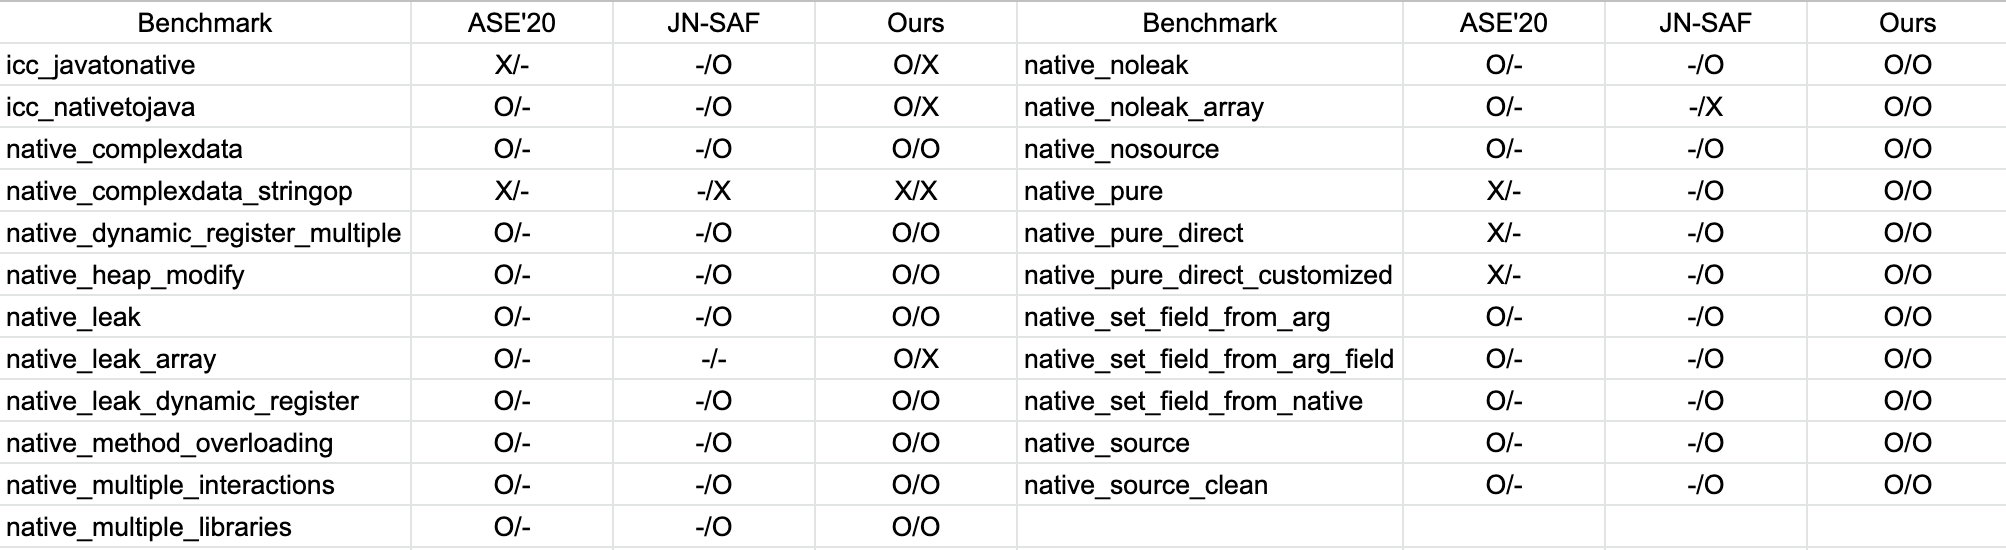
\includegraphics[width=0.5\textwidth]{img/table1}
The table1 shows the analysis result for 19 benchmarks in NativeFlowBench.  The
"Benchmark" coulmns denote the benchmark names, and "result" coulmns denote
whether the analysis result for corresponding benchmark was correct(O) or
not(X). We call that the analysis result is successful if every function call
target (call(j->c), call(c->j)) and field access tagret (field\_read(c->j),
field\_write(c->j)) are precisely determined, and every data leak is reported
correctly without false positives or false negatives.  The result shows that
except for one benchmark, our analyzer could correctly determine all targets
for function calls and field access correctly, and could successfully perform
dataflow analysis to find all of the data leaks. The only exception was
native\_compexdata\_stringop, where string manipulation functions such as
strcpy or strcat from C++'s standard library were used to create the string
value that indicates the target method's name, and since the inner-flow
analysis could not properly handle these functions, analyzer could not
correctly deterimine the function call target.

(Emphasize that data leak was not found in the previous research? or not?)

\subsection{RQ2: Performance}
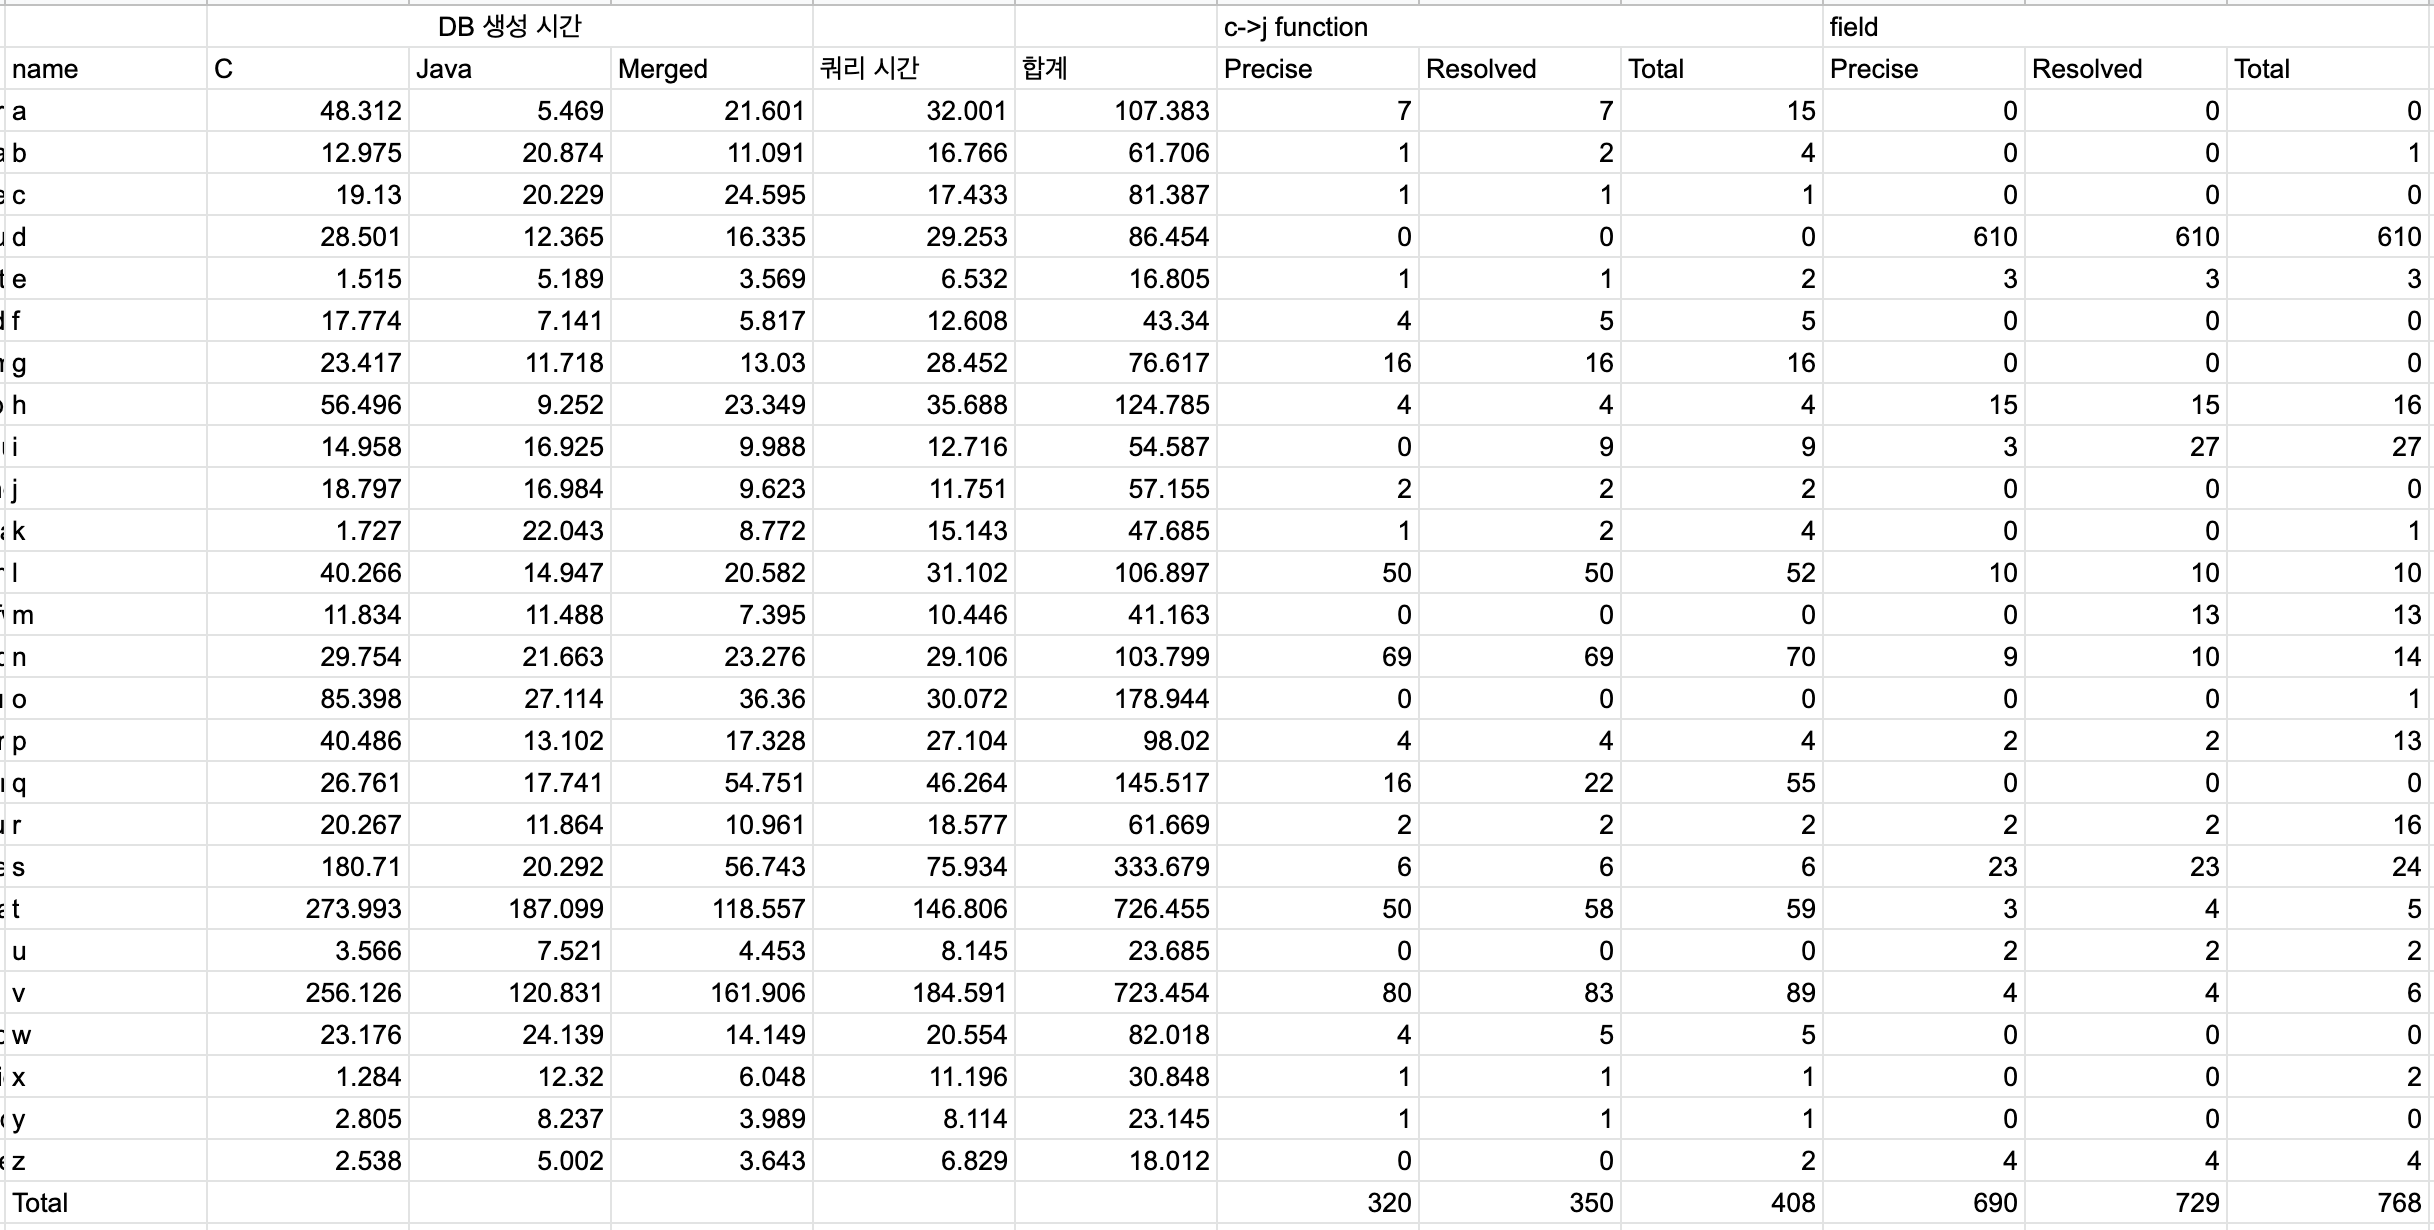
\includegraphics[width=0.5\textwidth]{img/table2}
The table2 shows the analysis result for 42 F-Droid applications. The "time"
coulmn denotes the time for creating database and evaluating query. The average
time for creating DB was ??? seconds, and average time for evaluating query was
??? seconds, making the total analysis time ??? seconds. This is x4 faster on
average, compared to the state-of-the art JNI program analyzer.  Note that time
for creating DB includes compile time, and once DB is created, multiple queries
can be evaluated withou creating DB again. This means that pratically, the
pratical speed up becomes x14.

The "precision" coulms denotes the precision of dispatching function call
target, and field access target.  "Precise" means exactly one target was found,
and resolved means at least one target was found.  Compared to the previous
result, the precision was also higher for both function call targets and field
access targets.

\subsection{RQ3: Usefulness}

